\documentclass[11pt]{article}

%
% Packages and settings for mimicking the Jupyter notebook's behavior
%
% \setcounter{secnumdepth}{0} %Suppress section numbers
%\usepackage{parskip} % Stop auto-indenting (to mimic markdown behaviour)
% \usepackage{longtable} % longtable support required by pandoc >1.10
% \usepackage{booktabs}  % table support for pandoc > 1.12.2
% \usepackage[inline]{enumitem} % IRkernel/repr support (it uses the enumerate* environment)
% \usepackage[normalem]{ulem} % ulem is needed to support strikethroughs (\sout)
%								% normalem makes italics be italics, not underlines
%
%

% The hyperref package gives us a pdf with properly built
% internal navigation ('pdf bookmarks' for the table of contents,
% internal cross-reference links, web links for URLs, etc.)
\usepackage{hyperref}
% The default LaTeX title has an obnoxious amount of whitespace. By default,
% titling removes some of it. It also provides customization options.
\usepackage{titling}

\usepackage{geometry} % Used to adjust the document margins
\usepackage{textcomp} % defines textquotesingle

\usepackage{parskip} % omit tab at the beginning of a new paragraph
\usepackage{upquote} % Upright quotes for verbatim code

% Figures and styles
%\usepackage[Export]{adjustbox} % Used to constrain images to a maximum size
\usepackage{float}
%\floatplacement{figure}{H} % forces figures to be placed at the correct location
\usepackage{graphicx} % Basic figure setup
%\usepackage{fancyvrb} % verbatim replacement that allows latex
\usepackage{grffile} % extends the file name processing of package graphics 

% Math
\usepackage{amsmath} % Equations
\usepackage{amssymb} % Equations
\usepackage{mathrsfs}
\usepackage[mathletters]{ucs} % Extended unicode (utf-8) support



%%
%% BEGIN DOCUMENT
%%
\begin{document}

\newcommand{\subtitle}[1]{%
  \posttitle{%
    \par\end{center}
    \begin{center}\large#1\end{center}
    \vskip0.5em}%
}

\title{Squared grid puzzle}
\subtitle{An informal analysis of the classical nine-dots puzzle ``under steroids''}
\date{}
\author{\\ Andrea Rebolini}

\maketitle

\begin{figure}[H]
\centering
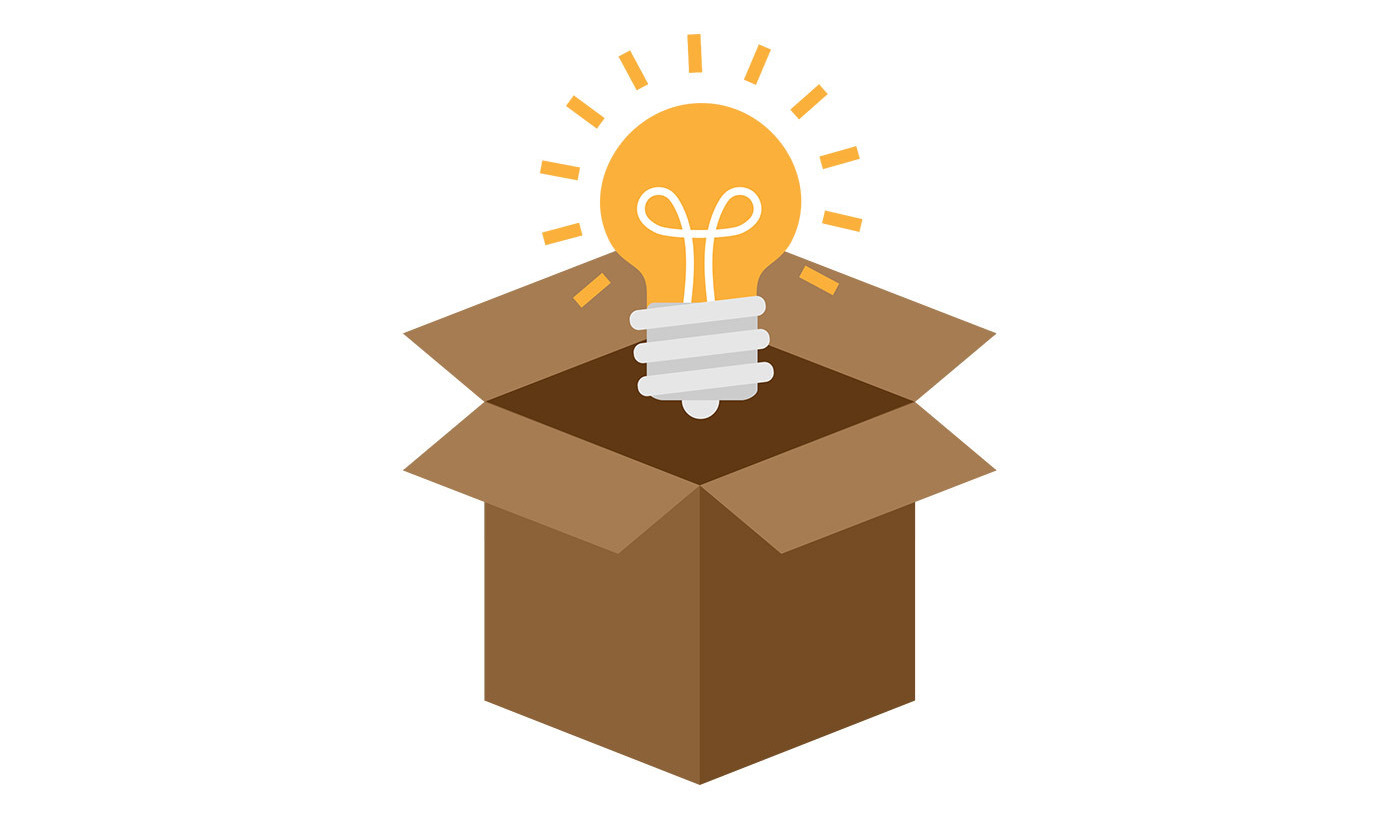
\includegraphics[width=0.4\textwidth]{images/think-out-the-box-icon.jpg}
\end{figure}

\begin{abstract}
The nine-dots puzzle is a mainstream brain-teaser. It's often sponsored by business coaches and salesmen as a benchmark of creative thinking, as its solution requires to ``think outside-the-box".
In this paper, I review the nine-dots puzzle and then analyze a generalized version of the original problem, which is extended to a squared grid consisting of an arbitrary number of points: i.e, the starting \emph{9-dots puzzle} becomes the generic \emph{9-16-25-36.. dots puzzle}. First, I show how the general solution can be achieved. You'll then learn that starting from a particular grid size upwards, salesmen can no longer enthrall you with out-of-the-box tricks. Finally, I propose an intriguing arithmetical interpretation of the solution to the general bidimensional problem.
\\
\\
\textbf{Disclaimer}: the squared grid problem has already been solved and thoroughly treated. Marco Ripà and Pablo Ramirez first extended the nine-dots puzzle to an arbitrarily-sized squared grid and then also to multiple dimensions! You can find their papers in the \hyperlink{references}{References} section.\\
This document simply aims to be an enjoyable and informal digression on the squared grid problem as posed by the aforementioned authors. As regards the arithmetical interpretation of the solution to the puzzle that I'll provide, so far I didn't find any counterpart by searching online but I may be wrong: in case it's an original remark, you're welcome!
\end{abstract}

\newpage

\hypertarget{nine-dots-puzzle} {
	\section{The nine dots puzzle}
	\label{nine-dots-puzzle}
}
The \textbf{nine-dots puzzle} has been first cited by Sam Loyd's in his \emph{Cyclopedia of Puzzles} (see \autoref{fig:egg_puzzle}).
\begin{figure}[H]
	\centering
	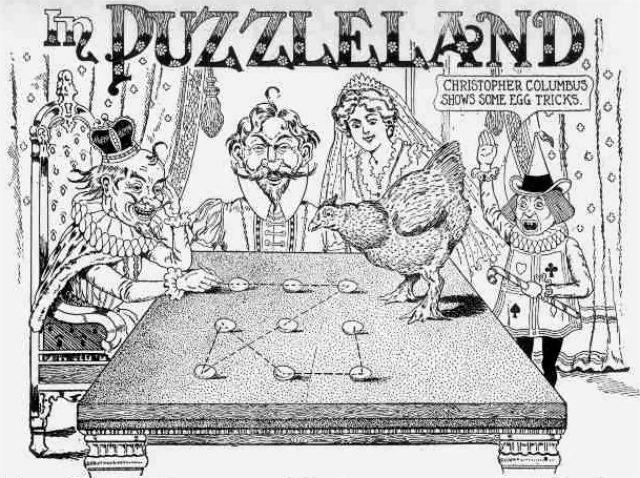
\includegraphics[width=0.54\textwidth]{images/egg_puzzle.jpg}
	\caption{The original illustration of the nine-dots puzzle in the Sam Loyd's "Cyclopedia of puzzle" (1914). The author entitled it as \emph{the Christoforus Columbus egg puzzle}; this is just a reference to the \emph{egg of Columbus}: you don't actually need 9 eggs to try it yourself.}
\label{fig:egg_puzzle}
\end{figure}
In its basic formulation, the goal is to join nine dots arranged in a squared grid with the fewest number of straight lines, and without lifting the pen. Take your time to figure out the solution...
\begin{figure}[H]
\centering
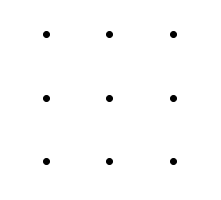
\includegraphics[width=0.3\textwidth]{images/9-dots-grid.png}
\caption{The 9-dots puzzle: join all the points using straight lines, without lifting the pen.}
\label{fig:9-dots-grid}
\end{figure}
If you concluded that at least five lines are required to join all the points, and your solution is something like \autoref{fig:9-dots-wrong} alas! you embraced mediocrity and should not complain about your pen-pusher job. But don't worry: contrast your outcome with the one given by the king in the Sam Loyd's illustration (again \autoref{fig:egg_puzzle}): you're ahead by one line against the king, and thus still highly qualified to rule a nation.
\begin{figure}[H]
\centering
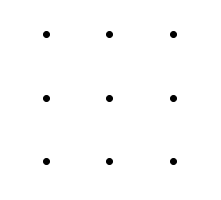
\includegraphics[width=0.3\textwidth]{images/9-dots-grid.png}
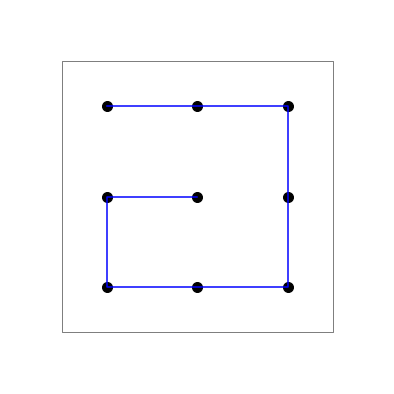
\includegraphics[width=0.3\textwidth]{images/9-dots-wrong-solution.png}
\caption{A suspiciously trivial (and thus wrong) solution to the 9-dots puzzle.}
\label{fig:9-dots-wrong}
\end{figure}
How is possible to connect the dots with fewer lines?
What hinders most of the people is that they restrict themselves to draw lines within the grid of points, myopically focusing on an immaginary boundary around the grid (similar to the thin grey borders that I maliciously put in the above figures). In order to get to the ``right" solution (or at least to a more optimal solution: in \hyperlink{appendices}{Appendices}, you'll see why I make such a clarification) you need to \textbf{``think outside the box''}. Using a more creative mindset, a solution can be drawn consisting of just four lines, as shown in \autoref{fig:9-dots-solution}.
%% TODO references to the figure's number are all wrong! But the links are correct.
\begin{figure}[H]
\centering
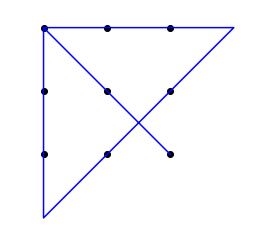
\includegraphics[width=0.3\textwidth]{images/9-dots-solution.png}
\caption{A creative and effective solution to the 9-dots puzzle. Think outside the box!}
\label{fig:9-dots-solution}
\end{figure}
Nice trick, isn't it?! No surprise, this intriguing conundrum was revived by psychologists, salesmen and business coaches, always seeking a nice \emph{coup-de-théâtre} for their demonstrations.


\hypertarget{the-extended-problem-and-its-solution} {
	\section{The extended problem and its solution}
	\label{the-extended-problem-and-its-solution}
}
%
%First, I'll show that the general solution can be drawn iteratively, as you may have already guessed

\hypertarget{final-notes}{
	\section{Final notes}
	\label{final-notes}
}

\paragraph{Acknowledgements} \mbox{} \\ % mbox needed for having carriage return after "paragraph"
Marco Ripà posed the squared grid brain-teaser during one of its stimulating \href{https://www.youtube.com/watch?v=rh-ONRXcHok}{YouTube live sessions}. I am obliged to him for the great fun I had in tackling this problem, which in turn inspired all the analysis and ideas that followed.

\paragraph{Technical note for computer nerds} \mbox{} \\
Python was used to code the solver algorithm and produce the explanatory images of the paper. You can find the implementation in the attached Jupyter notebook, in which you can also display (and save) a nice animation drawing the solution to the puzzle.

\paragraph{Future developments} \mbox{} \\
I'll address the problem in multiple dimensions, you bet! I would also like to extend the solver's code to handle this more general case; hence, as a plus I could produce animations drawing the solution for three-dimensional grids.

\hypertarget{appendices}{
	\section{Appendices}
	\label{appendices}
}

\hypertarget{references}{
	\section{References}
	\label{references}
}

\begin{itemize}
	\item
		The basic nine-dots puzzle has been first cited here: \emph{Cyclopedia of Puzzles, Samuel Loyd (1914)}.
	\item
	\href{https://en.wikipedia.org/wiki/Thinking_outside_the_box}{Wikipedia page on out-of-the-box thinking} is worth reading: the 9-dots puzzle is thoroughly discussed.
	\item
		A link to a really valid \href{http://utenti.quipo.it/base5/geopiana/loyd9punti4linee.htm}{online reference (in Italian)}
	\item
		\emph{Marco Ripà and Pablo Ramirez, Il Nine Dots Puzzle esteso a N×N×\ldots×N punti}.
	\item
		\emph{Marco Ripà, Nine Dots Puzzle extended to N1×N2×\ldots×Nk points 	under house arrest}.
\end{itemize}

\end{document}
